%%%%%%%%%%%%%%%%%%%%%%%%%%%%%%%%%%%%%%%%%
% Masters/Doctoral Thesis 
% LaTeX Template
% Version 2.4 (22/11/16)
%
% This template has been downloaded from:
% http://www.LaTeXTemplates.com
%
% Version 2.x major modifications by:
% Vel (vel@latextemplates.com)
%
% This template is based on a template by:
% Steve Gunn (http://users.ecs.soton.ac.uk/srg/softwaretools/document/templates/)
% Sunil Patel (http://www.sunilpatel.co.uk/thesis-template/)
%
% Template license:
% CC BY-NC-SA 3.0 (http://creativecommons.org/licenses/by-nc-sa/3.0/)
%
%%%%%%%%%%%%%%%%%%%%%%%%%%%%%%%%%%%%%%%%%

%----------------------------------------------------------------------------------------
%	PACKAGES AND OTHER DOCUMENT CONFIGURATIONS
%----------------------------------------------------------------------------------------

\documentclass[
11pt, % The default document font size, options: 10pt, 11pt, 12pt
%oneside, % Two side (alternating margins) for binding by default, uncomment to switch to one side
english, % ngerman for German
onehalfspacing, % Single line spacing, alternatives: onehalfspacing or doublespacing
%draft, % Uncomment to enable draft mode (no pictures, no links, overfull hboxes indicated)
%nolistspacing, % If the document is onehalfspacing or doublespacing, uncomment this to set spacing in lists to single
%liststotoc, % Uncomment to add the list of figures/tables/etc to the table of contents
%toctotoc, % Uncomment to add the main table of contents to the table of contents
%parskip, % Uncomment to add space between paragraphs
%nohyperref, % Uncomment to not load the hyperref package
%headsepline, % Uncomment to get a line under the header
%chapterinoneline, % Uncomment to place the chapter title next to the number on one line
%consistentlayout, % Uncomment to change the layout of the declaration, abstract and acknowledgements pages to match the default layout
]{MastersDoctoralThesis} % The class file specifying the document structure

\usepackage[utf8]{inputenc} % Required for inputting international characters
\usepackage[T1]{fontenc} % Output font encoding for international characters

\usepackage{palatino} % Use the Palatino font by default

\usepackage[backend=bibtex,style=authoryear,natbib=true]{biblatex} % Use the bibtex backend with the authoryear citation style (which resembles APA)

\addbibresource{example.bib} % The filename of the bibliography

\usepackage[autostyle=true]{csquotes} % Required to generate language-dependent quotes in the bibliography

%----------------------------------------------------------------------------------------
%	MARGIN SETTINGS
%----------------------------------------------------------------------------------------

\geometry{
	paper=letterpaper, % Change to letterpaper for US letter
	inner=2.5cm, % Inner margin
	outer=3.8cm, % Outer margin
	bindingoffset=.5cm, % Binding offset
	top=3.5cm, % Top margin
	bottom=3cm, % Bottom margin
	%showframe, % Uncomment to show how the type block is set on the page
}

%----------------------------------------------------------------------------------------
%	THESIS INFORMATION
%----------------------------------------------------------------------------------------

\thesistitle{Big Data Streaming} % Your thesis title, this is used in the title and abstract, print it elsewhere with \ttitle
\supervisor{Dott. Luca \textsc{Oneto}} % Your supervisor's name, this is used in the title page, print it elsewhere with \supname
\examiner{} % Your examiner's name, this is not currently used anywhere in the template, print it elsewhere with \examname
\degree{Corso di Studio in Ingegneria Informatica} % Your degree name, this is used in the title page and abstract, print it elsewhere with \degreename
\author{Federico \textsc{D'Ambrosio}} % Your name, this is used in the title page and abstract, print it elsewhere with \authorname
\addresses{} % Your address, this is not currently used anywhere in the template, print it elsewhere with \addressname

\subject{Data Analysis} % Your subject area, this is not currently used anywhere in the template, print it elsewhere with \subjectname
\keywords{} % Keywords for your thesis, this is not currently used anywhere in the template, print it elsewhere with \keywordnames
\university{{Università degli studi di Genova}} % Your university's name and URL, this is used in the title page and abstract, print it elsewhere with \univname
\department{\href{http://www.dibris.unige.it/}{Dibris}} % Your department's name and URL, this is used in the title page and abstract, print it elsewhere with \deptname
\group{\href{http://researchgroup.university.com}{Research Group Name}} % Your research group's name and URL, this is used in the title page, print it elsewhere with \groupname
\faculty{\href{http://www.informatica.ingegneria.unige.it/}{Ingegneria Informatica}} % Your faculty's name and URL, this is used in the title page and abstract, print it elsewhere with \facname

\AtBeginDocument{
\hypersetup{pdftitle=\ttitle} % Set the PDF's title to your title
\hypersetup{pdfauthor=\authorname} % Set the PDF's author to your name
\hypersetup{pdfkeywords=\keywordnames} % Set the PDF's keywords to your keywords
}

\begin{document}

\frontmatter % Use roman page numbering style (i, ii, iii, iv...) for the pre-content pages

\pagestyle{plain} % Default to the plain heading style until the thesis style is called for the body content

%----------------------------------------------------------------------------------------
%	TITLE PAGE
%----------------------------------------------------------------------------------------

\begin{titlepage}
%\linespread{1.5}
\thispagestyle{empty}
\begin{center}
	
\includegraphics[width=0.2\linewidth]{Figures/unige.eps}
\end{center}

\begin{center}
	\LARGE\sc
	\univname\\
	
	\vspace{0.5cm}
	\large
	\degreename\\
\end{center}

\begin{center}
	\small
	Tesi di Laurea per il conseguimento del titolo di\\
	Dottore Magistrale in Ingegneria Informatica\\
\end{center}

\vfill

\begin{center} 
	\LARGE
	{\bf \ttitle}\\
	\vspace{0.5cm}
	\large
	\authorname\\
	\vspace{0.5cm}
	\small
	Dicembre 2017
\end{center}

\vfill

\begin{tabular}{lll}%
	{\em Relatore}:	& Prof.	& Luca Oneto\\
	{\em Correlatore}:	& Dott.	& Nome Cognome\\
\end{tabular} 

\hfill


\end{titlepage}

%----------------------------------------------------------------------------------------
%	DECLARATION PAGE
%----------------------------------------------------------------------------------------

\begin{declaration}
\addchaptertocentry{\authorshipname} % Add the declaration to the table of contents
\noindent I, \authorname, declare that this thesis titled, \enquote{\ttitle} and the work presented in it are my own. I confirm that:

\begin{itemize} 
\item This work was done wholly or mainly while in candidature for a research degree at this University.
\item Where any part of this thesis has previously been submitted for a degree or any other qualification at this University or any other institution, this has been clearly stated.
\item Where I have consulted the published work of others, this is always clearly attributed.
\item Where I have quoted from the work of others, the source is always given. With the exception of such quotations, this thesis is entirely my own work.
\item I have acknowledged all main sources of help.
\item Where the thesis is based on work done by myself jointly with others, I have made clear exactly what was done by others and what I have contributed myself.\\
\end{itemize}
 
\noindent Signed:\\
\rule[0.5em]{25em}{0.5pt} % This prints a line for the signature
 
\noindent Date:\\
\rule[0.5em]{25em}{0.5pt} % This prints a line to write the date
\end{declaration}

\cleardoublepage

%----------------------------------------------------------------------------------------
%	QUOTATION PAGE
%----------------------------------------------------------------------------------------

\vspace*{0.2\textheight}

\noindent\enquote{\itshape Thanks to my solid academic training, today I can write hundreds of words on virtually any topic without possessing a shred of information, which is how I got a good job in journalism.}\bigbreak

\hfill Dave Barry

%----------------------------------------------------------------------------------------
%	ABSTRACT PAGE
%----------------------------------------------------------------------------------------

\begin{abstract}
\addchaptertocentry{\abstractname} % Add the abstract to the table of contents
The Thesis Abstract is written here (and usually kept to just this page). The page is kept centered vertically so can expand into the blank space above the title too\ldots
\end{abstract}

%----------------------------------------------------------------------------------------
%	ACKNOWLEDGEMENTS
%----------------------------------------------------------------------------------------

\begin{acknowledgements}
\addchaptertocentry{\acknowledgementname} % Add the acknowledgements to the table of contents
The acknowledgments and the people to thank go here, don't forget to include your project advisor\ldots
\end{acknowledgements}

%----------------------------------------------------------------------------------------
%	LIST OF CONTENTS/FIGURES/TABLES PAGES
%----------------------------------------------------------------------------------------

\tableofcontents % Prints the main table of contents

\listoffigures % Prints the list of figures

\listoftables % Prints the list of tables

%----------------------------------------------------------------------------------------
%	ABBREVIATIONS
%----------------------------------------------------------------------------------------

\begin{abbreviations}{ll} % Include a list of abbreviations (a table of two columns)

\textbf{LAH} & \textbf{L}ist \textbf{A}bbreviations \textbf{H}ere\\
\textbf{WSF} & \textbf{W}hat (it) \textbf{S}tands \textbf{F}or\\

\end{abbreviations}

%----------------------------------------------------------------------------------------
%	PHYSICAL CONSTANTS/OTHER DEFINITIONS
%----------------------------------------------------------------------------------------

\begin{constants}{lr@{${}={}$}l} % The list of physical constants is a three column table

% The \SI{}{} command is provided by the siunitx package, see its documentation for instructions on how to use it

Speed of Light & $c_{0}$ & \SI{2.99792458e8}{\meter\per\second} (exact)\\
%Constant Name & $Symbol$ & $Constant Value$ with units\\

\end{constants}

%----------------------------------------------------------------------------------------
%	SYMBOLS
%----------------------------------------------------------------------------------------

\begin{symbols}{lll} % Include a list of Symbols (a three column table)

$a$ & distance & \si{\meter} \\
$P$ & power & \si{\watt} (\si{\joule\per\second}) \\
%Symbol & Name & Unit \\

\addlinespace % Gap to separate the Roman symbols from the Greek

$\omega$ & angular frequency & \si{\radian} \\

\end{symbols}

%----------------------------------------------------------------------------------------
%	DEDICATION
%----------------------------------------------------------------------------------------

\dedicatory{For/Dedicated to/To my\ldots} 

%----------------------------------------------------------------------------------------
%	THESIS CONTENT - CHAPTERS
%----------------------------------------------------------------------------------------

\mainmatter % Begin numeric (1,2,3...) page numbering

\pagestyle{thesis} % Return the page headers back to the "thesis" style

% Include the chapters of the thesis as separate files from the Chapters folder
% Uncomment the lines as you write the chapters

% Chapter 1

\chapter{Chapter Title Here} % Main chapter title

\label{Chapter1} % For referencing the chapter elsewhere, use \ref{Chapter1} 

%----------------------------------------------------------------------------------------

% Define some commands to keep the formatting separated from the content 
\newcommand{\keyword}[1]{\textbf{#1}}
\newcommand{\tabhead}[1]{\textbf{#1}}
\newcommand{\code}[1]{\texttt{#1}}
\newcommand{\file}[1]{\texttt{\bfseries#1}}
\newcommand{\option}[1]{\texttt{\itshape#1}}

%----------------------------------------------------------------------------------------

\section{Welcome and Thank You}
Welcome to this \LaTeX{} Thesis Template, a beautiful and easy to use template for writing a thesis using the \LaTeX{} typesetting system.

If you are writing a thesis (or will be in the future) and its subject is technical or mathematical (though it doesn't have to be), then creating it in \LaTeX{} is highly recommended as a way to make sure you can just get down to the essential writing without having to worry over formatting or wasting time arguing with your word processor.

\LaTeX{} is easily able to professionally typeset documents that run to hundreds or thousands of pages long. With simple mark-up commands, it automatically sets out the table of contents, margins, page headers and footers and keeps the formatting consistent and beautiful. One of its main strengths is the way it can easily typeset mathematics, even \emph{heavy} mathematics. Even if those equations are the most horribly twisted and most difficult mathematical problems that can only be solved on a super-computer, you can at least count on \LaTeX{} to make them look stunning.

%----------------------------------------------------------------------------------------

\section{Learning \LaTeX{}}

\LaTeX{} is not a \textsc{wysiwyg} (What You See is What You Get) program, unlike word processors such as Microsoft Word or Apple's Pages. Instead, a document written for \LaTeX{} is actually a simple, plain text file that contains \emph{no formatting}. You tell \LaTeX{} how you want the formatting in the finished document by writing in simple commands amongst the text, for example, if I want to use \emph{italic text for emphasis}, I write the \verb|\emph{text}| command and put the text I want in italics in between the curly braces. This means that \LaTeX{} is a \enquote{mark-up} language, very much like HTML.

\subsection{A (not so short) Introduction to \LaTeX{}}

If you are new to \LaTeX{}, there is a very good eBook -- freely available online as a PDF file -- called, \enquote{The Not So Short Introduction to \LaTeX{}}. The book's title is typically shortened to just \emph{lshort}. You can download the latest version (as it is occasionally updated) from here:
\url{http://www.ctan.org/tex-archive/info/lshort/english/lshort.pdf}

It is also available in several other languages. Find yours from the list on this page: \url{http://www.ctan.org/tex-archive/info/lshort/}

It is recommended to take a little time out to learn how to use \LaTeX{} by creating several, small `test' documents, or having a close look at several templates on:\\ 
\url{http://www.LaTeXTemplates.com}\\ 
Making the effort now means you're not stuck learning the system when what you \emph{really} need to be doing is writing your thesis.

\subsection{A Short Math Guide for \LaTeX{}}

If you are writing a technical or mathematical thesis, then you may want to read the document by the AMS (American Mathematical Society) called, \enquote{A Short Math Guide for \LaTeX{}}. It can be found online here:
\url{http://www.ams.org/tex/amslatex.html}
under the \enquote{Additional Documentation} section towards the bottom of the page.

\subsection{Common \LaTeX{} Math Symbols}
There are a multitude of mathematical symbols available for \LaTeX{} and it would take a great effort to learn the commands for them all. The most common ones you are likely to use are shown on this page:
\url{http://www.sunilpatel.co.uk/latex-type/latex-math-symbols/}

You can use this page as a reference or crib sheet, the symbols are rendered as large, high quality images so you can quickly find the \LaTeX{} command for the symbol you need.

\subsection{\LaTeX{} on a Mac}
 
The \LaTeX{} distribution is available for many systems including Windows, Linux and Mac OS X. The package for OS X is called MacTeX and it contains all the applications you need -- bundled together and pre-customized -- for a fully working \LaTeX{} environment and work flow.
 
MacTeX includes a custom dedicated \LaTeX{} editor called TeXShop for writing your `\file{.tex}' files and BibDesk: a program to manage your references and create your bibliography section just as easily as managing songs and creating playlists in iTunes.

%----------------------------------------------------------------------------------------

\section{Getting Started with this Template}

If you are familiar with \LaTeX{}, then you should explore the directory structure of the template and then proceed to place your own information into the \emph{THESIS INFORMATION} block of the \file{main.tex} file. You can then modify the rest of this file to your unique specifications based on your degree/university. Section \ref{FillingFile} on page \pageref{FillingFile} will help you do this. Make sure you also read section \ref{ThesisConventions} about thesis conventions to get the most out of this template.

If you are new to \LaTeX{} it is recommended that you carry on reading through the rest of the information in this document.

Before you begin using this template you should ensure that its style complies with the thesis style guidelines imposed by your institution. In most cases this template style and layout will be suitable. If it is not, it may only require a small change to bring the template in line with your institution's recommendations. These modifications will need to be done on the \file{MastersDoctoralThesis.cls} file.

\subsection{About this Template}

This \LaTeX{} Thesis Template is originally based and created around a \LaTeX{} style file created by Steve R.\ Gunn from the University of Southampton (UK), department of Electronics and Computer Science. You can find his original thesis style file at his site, here:
\url{http://www.ecs.soton.ac.uk/~srg/softwaretools/document/templates/}

Steve's \file{ecsthesis.cls} was then taken by Sunil Patel who modified it by creating a skeleton framework and folder structure to place the thesis files in. The resulting template can be found on Sunil's site here:
\url{http://www.sunilpatel.co.uk/thesis-template}

Sunil's template was made available through \url{http://www.LaTeXTemplates.com} where it was modified many times based on user requests and questions. Version 2.0 and onwards of this template represents a major modification to Sunil's template and is, in fact, hardly recognisable. The work to make version 2.0 possible was carried out by \href{mailto:vel@latextemplates.com}{Vel} and Johannes Böttcher.

%----------------------------------------------------------------------------------------

\section{What this Template Includes}

\subsection{Folders}

This template comes as a single zip file that expands out to several files and folders. The folder names are mostly self-explanatory:

\keyword{Appendices} -- this is the folder where you put the appendices. Each appendix should go into its own separate \file{.tex} file. An example and template are included in the directory.

\keyword{Chapters} -- this is the folder where you put the thesis chapters. A thesis usually has about six chapters, though there is no hard rule on this. Each chapter should go in its own separate \file{.tex} file and they can be split as:
\begin{itemize}
\item Chapter 1: Introduction to the thesis topic
\item Chapter 2: Background information and theory
\item Chapter 3: (Laboratory) experimental setup
\item Chapter 4: Details of experiment 1
\item Chapter 5: Details of experiment 2
\item Chapter 6: Discussion of the experimental results
\item Chapter 7: Conclusion and future directions
\end{itemize}
This chapter layout is specialised for the experimental sciences, your discipline may be different.

\keyword{Figures} -- this folder contains all figures for the thesis. These are the final images that will go into the thesis document.

\subsection{Files}

Included are also several files, most of them are plain text and you can see their contents in a text editor. After initial compilation, you will see that more auxiliary files are created by \LaTeX{} or BibTeX and which you don't need to delete or worry about:

\keyword{example.bib} -- this is an important file that contains all the bibliographic information and references that you will be citing in the thesis for use with BibTeX. You can write it manually, but there are reference manager programs available that will create and manage it for you. Bibliographies in \LaTeX{} are a large subject and you may need to read about BibTeX before starting with this. Many modern reference managers will allow you to export your references in BibTeX format which greatly eases the amount of work you have to do.

\keyword{MastersDoctoralThesis.cls} -- this is an important file. It is the class file that tells \LaTeX{} how to format the thesis. 

\keyword{main.pdf} -- this is your beautifully typeset thesis (in the PDF file format) created by \LaTeX{}. It is supplied in the PDF with the template and after you compile the template you should get an identical version.

\keyword{main.tex} -- this is an important file. This is the file that you tell \LaTeX{} to compile to produce your thesis as a PDF file. It contains the framework and constructs that tell \LaTeX{} how to layout the thesis. It is heavily commented so you can read exactly what each line of code does and why it is there. After you put your own information into the \emph{THESIS INFORMATION} block -- you have now started your thesis!

Files that are \emph{not} included, but are created by \LaTeX{} as auxiliary files include:

\keyword{main.aux} -- this is an auxiliary file generated by \LaTeX{}, if it is deleted \LaTeX{} simply regenerates it when you run the main \file{.tex} file.

\keyword{main.bbl} -- this is an auxiliary file generated by BibTeX, if it is deleted, BibTeX simply regenerates it when you run the \file{main.aux} file. Whereas the \file{.bib} file contains all the references you have, this \file{.bbl} file contains the references you have actually cited in the thesis and is used to build the bibliography section of the thesis.

\keyword{main.blg} -- this is an auxiliary file generated by BibTeX, if it is deleted BibTeX simply regenerates it when you run the main \file{.aux} file.

\keyword{main.lof} -- this is an auxiliary file generated by \LaTeX{}, if it is deleted \LaTeX{} simply regenerates it when you run the main \file{.tex} file. It tells \LaTeX{} how to build the \emph{List of Figures} section.

\keyword{main.log} -- this is an auxiliary file generated by \LaTeX{}, if it is deleted \LaTeX{} simply regenerates it when you run the main \file{.tex} file. It contains messages from \LaTeX{}, if you receive errors and warnings from \LaTeX{}, they will be in this \file{.log} file.

\keyword{main.lot} -- this is an auxiliary file generated by \LaTeX{}, if it is deleted \LaTeX{} simply regenerates it when you run the main \file{.tex} file. It tells \LaTeX{} how to build the \emph{List of Tables} section.

\keyword{main.out} -- this is an auxiliary file generated by \LaTeX{}, if it is deleted \LaTeX{} simply regenerates it when you run the main \file{.tex} file.

So from this long list, only the files with the \file{.bib}, \file{.cls} and \file{.tex} extensions are the most important ones. The other auxiliary files can be ignored or deleted as \LaTeX{} and BibTeX will regenerate them.

%----------------------------------------------------------------------------------------

\section{Filling in Your Information in the \file{main.tex} File}\label{FillingFile}

You will need to personalise the thesis template and make it your own by filling in your own information. This is done by editing the \file{main.tex} file in a text editor or your favourite LaTeX environment.

Open the file and scroll down to the third large block titled \emph{THESIS INFORMATION} where you can see the entries for \emph{University Name}, \emph{Department Name}, etc \ldots

Fill out the information about yourself, your group and institution. You can also insert web links, if you do, make sure you use the full URL, including the \code{http://} for this. If you don't want these to be linked, simply remove the \verb|\href{url}{name}| and only leave the name.

When you have done this, save the file and recompile \code{main.tex}. All the information you filled in should now be in the PDF, complete with web links. You can now begin your thesis proper!

%----------------------------------------------------------------------------------------

\section{The \code{main.tex} File Explained}

The \file{main.tex} file contains the structure of the thesis. There are plenty of written comments that explain what pages, sections and formatting the \LaTeX{} code is creating. Each major document element is divided into commented blocks with titles in all capitals to make it obvious what the following bit of code is doing. Initially there seems to be a lot of \LaTeX{} code, but this is all formatting, and it has all been taken care of so you don't have to do it.

Begin by checking that your information on the title page is correct. For the thesis declaration, your institution may insist on something different than the text given. If this is the case, just replace what you see with what is required in the \emph{DECLARATION PAGE} block.

Then comes a page which contains a funny quote. You can put your own, or quote your favourite scientist, author, person, and so on. Make sure to put the name of the person who you took the quote from.

Following this is the abstract page which summarises your work in a condensed way and can almost be used as a standalone document to describe what you have done. The text you write will cause the heading to move up so don't worry about running out of space.

Next come the acknowledgements. On this page, write about all the people who you wish to thank (not forgetting parents, partners and your advisor/supervisor).

The contents pages, list of figures and tables are all taken care of for you and do not need to be manually created or edited. The next set of pages are more likely to be optional and can be deleted since they are for a more technical thesis: insert a list of abbreviations you have used in the thesis, then a list of the physical constants and numbers you refer to and finally, a list of mathematical symbols used in any formulae. Making the effort to fill these tables means the reader has a one-stop place to refer to instead of searching the internet and references to try and find out what you meant by certain abbreviations or symbols.

The list of symbols is split into the Roman and Greek alphabets. Whereas the abbreviations and symbols ought to be listed in alphabetical order (and this is \emph{not} done automatically for you) the list of physical constants should be grouped into similar themes.

The next page contains a one line dedication. Who will you dedicate your thesis to?

Finally, there is the block where the chapters are included. Uncomment the lines (delete the \code{\%} character) as you write the chapters. Each chapter should be written in its own file and put into the \emph{Chapters} folder and named \file{Chapter1}, \file{Chapter2}, etc\ldots Similarly for the appendices, uncomment the lines as you need them. Each appendix should go into its own file and placed in the \emph{Appendices} folder.

After the preamble, chapters and appendices finally comes the bibliography. The bibliography style (called \option{authoryear}) is used for the bibliography and is a fully featured style that will even include links to where the referenced paper can be found online. Do not underestimate how grateful your reader will be to find that a reference to a paper is just a click away. Of course, this relies on you putting the URL information into the BibTeX file in the first place.

%----------------------------------------------------------------------------------------

\section{Thesis Features and Conventions}\label{ThesisConventions}

To get the best out of this template, there are a few conventions that you may want to follow.

One of the most important (and most difficult) things to keep track of in such a long document as a thesis is consistency. Using certain conventions and ways of doing things (such as using a Todo list) makes the job easier. Of course, all of these are optional and you can adopt your own method.

\subsection{Printing Format}

This thesis template is designed for double sided printing (i.e. content on the front and back of pages) as most theses are printed and bound this way. Switching to one sided printing is as simple as uncommenting the \option{oneside} option of the \code{documentclass} command at the top of the \file{main.tex} file. You may then wish to adjust the margins to suit specifications from your institution.

The headers for the pages contain the page number on the outer side (so it is easy to flick through to the page you want) and the chapter name on the inner side.

The text is set to 11 point by default with single line spacing, again, you can tune the text size and spacing should you want or need to using the options at the very start of \file{main.tex}. The spacing can be changed similarly by replacing the \option{singlespacing} with \option{onehalfspacing} or \option{doublespacing}.

\subsection{Using US Letter Paper}

The paper size used in the template is A4, which is the standard size in Europe. If you are using this thesis template elsewhere and particularly in the United States, then you may have to change the A4 paper size to the US Letter size. This can be done in the margins settings section in \file{main.tex}.

Due to the differences in the paper size, the resulting margins may be different to what you like or require (as it is common for institutions to dictate certain margin sizes). If this is the case, then the margin sizes can be tweaked by modifying the values in the same block as where you set the paper size. Now your document should be set up for US Letter paper size with suitable margins.

\subsection{References}

The \code{biblatex} package is used to format the bibliography and inserts references such as this one \parencite{Reference1}. The options used in the \file{main.tex} file mean that the in-text citations of references are formatted with the author(s) listed with the date of the publication. Multiple references are separated by semicolons (e.g. \parencite{Reference2, Reference1}) and references with more than three authors only show the first author with \emph{et al.} indicating there are more authors (e.g. \parencite{Reference3}). This is done automatically for you. To see how you use references, have a look at the \file{Chapter1.tex} source file. Many reference managers allow you to simply drag the reference into the document as you type.

Scientific references should come \emph{before} the punctuation mark if there is one (such as a comma or period). The same goes for footnotes\footnote{Such as this footnote, here down at the bottom of the page.}. You can change this but the most important thing is to keep the convention consistent throughout the thesis. Footnotes themselves should be full, descriptive sentences (beginning with a capital letter and ending with a full stop). The APA6 states: \enquote{Footnote numbers should be superscripted, [...], following any punctuation mark except a dash.} The Chicago manual of style states: \enquote{A note number should be placed at the end of a sentence or clause. The number follows any punctuation mark except the dash, which it precedes. It follows a closing parenthesis.}

The bibliography is typeset with references listed in alphabetical order by the first author's last name. This is similar to the APA referencing style. To see how \LaTeX{} typesets the bibliography, have a look at the very end of this document (or just click on the reference number links in in-text citations).

\subsubsection{A Note on bibtex}

The bibtex backend used in the template by default does not correctly handle unicode character encoding (i.e. "international" characters). You may see a warning about this in the compilation log and, if your references contain unicode characters, they may not show up correctly or at all. The solution to this is to use the biber backend instead of the outdated bibtex backend. This is done by finding this in \file{main.tex}: \option{backend=bibtex} and changing it to \option{backend=biber}. You will then need to delete all auxiliary BibTeX files and navigate to the template directory in your terminal (command prompt). Once there, simply type \code{biber main} and biber will compile your bibliography. You can then compile \file{main.tex} as normal and your bibliography will be updated. An alternative is to set up your LaTeX editor to compile with biber instead of bibtex, see \href{http://tex.stackexchange.com/questions/154751/biblatex-with-biber-configuring-my-editor-to-avoid-undefined-citations/}{here} for how to do this for various editors.

\subsection{Tables}

Tables are an important way of displaying your results, below is an example table which was generated with this code:

{\small
\begin{verbatim}
\begin{table}
\caption{The effects of treatments X and Y on the four groups studied.}
\label{tab:treatments}
\centering
\begin{tabular}{l l l}
\toprule
\tabhead{Groups} & \tabhead{Treatment X} & \tabhead{Treatment Y} \\
\midrule
1 & 0.2 & 0.8\\
2 & 0.17 & 0.7\\
3 & 0.24 & 0.75\\
4 & 0.68 & 0.3\\
\bottomrule\\
\end{tabular}
\end{table}
\end{verbatim}
}

\begin{table}
\caption{The effects of treatments X and Y on the four groups studied.}
\label{tab:treatments}
\centering
\begin{tabular}{l l l}
\toprule
\tabhead{Groups} & \tabhead{Treatment X} & \tabhead{Treatment Y} \\
\midrule
1 & 0.2 & 0.8\\
2 & 0.17 & 0.7\\
3 & 0.24 & 0.75\\
4 & 0.68 & 0.3\\
\bottomrule\\
\end{tabular}
\end{table}

You can reference tables with \verb|\ref{<label>}| where the label is defined within the table environment. See \file{Chapter1.tex} for an example of the label and citation (e.g. Table~\ref{tab:treatments}).

\subsection{Figures}

There will hopefully be many figures in your thesis (that should be placed in the \emph{Figures} folder). The way to insert figures into your thesis is to use a code template like this:
\begin{verbatim}
\begin{figure}
\centering

\includegraphics{Figures/Electron.pdf}
\decoRule
\caption[An Electron]{An electron (artist's impression).}
\label{fig:Electron}
\end{figure}
\end{verbatim}
Also look in the source file. Putting this code into the source file produces the picture of the electron that you can see in the figure below.

\begin{figure}[th]
\centering

\includegraphics{Figures/Electron.pdf}
\decoRule
\caption[An Electron]{An electron (artist's impression).}
\label{fig:Electron}
\end{figure}

Sometimes figures don't always appear where you write them in the source. The placement depends on how much space there is on the page for the figure. Sometimes there is not enough room to fit a figure directly where it should go (in relation to the text) and so \LaTeX{} puts it at the top of the next page. Positioning figures is the job of \LaTeX{} and so you should only worry about making them look good!

Figures usually should have captions just in case you need to refer to them (such as in Figure~\ref{fig:Electron}). The \verb|\caption| command contains two parts, the first part, inside the square brackets is the title that will appear in the \emph{List of Figures}, and so should be short. The second part in the curly brackets should contain the longer and more descriptive caption text.

The \verb|\decoRule| command is optional and simply puts an aesthetic horizontal line below the image. If you do this for one image, do it for all of them.

\LaTeX{} is capable of using images in pdf, jpg and png format.

\subsection{Typesetting mathematics}

If your thesis is going to contain heavy mathematical content, be sure that \LaTeX{} will make it look beautiful, even though it won't be able to solve the equations for you.

The \enquote{Not So Short Introduction to \LaTeX} (available on \href{http://www.ctan.org/tex-archive/info/lshort/english/lshort.pdf}{CTAN}) should tell you everything you need to know for most cases of typesetting mathematics. If you need more information, a much more thorough mathematical guide is available from the AMS called, \enquote{A Short Math Guide to \LaTeX} and can be downloaded from:
\url{ftp://ftp.ams.org/pub/tex/doc/amsmath/short-math-guide.pdf}

There are many different \LaTeX{} symbols to remember, luckily you can find the most common symbols in \href{http://ctan.org/pkg/comprehensive}{The Comprehensive \LaTeX~Symbol List}.

You can write an equation, which is automatically given an equation number by \LaTeX{} like this:
\begin{verbatim}
\begin{equation}
E = mc^{2}
\label{eqn:Einstein}
\end{equation}
\end{verbatim}

This will produce Einstein's famous energy-matter equivalence equation:
\begin{equation}
E = mc^{2}
\label{eqn:Einstein}
\end{equation}

All equations you write (which are not in the middle of paragraph text) are automatically given equation numbers by \LaTeX{}. If you don't want a particular equation numbered, use the unnumbered form:
\begin{verbatim}
\[ a^{2}=4 \]
\end{verbatim}

%----------------------------------------------------------------------------------------

\section{Sectioning and Subsectioning}

You should break your thesis up into nice, bite-sized sections and subsections. \LaTeX{} automatically builds a table of Contents by looking at all the \verb|\chapter{}|, \verb|\section{}|  and \verb|\subsection{}| commands you write in the source.

The Table of Contents should only list the sections to three (3) levels. A \verb|chapter{}| is level zero (0). A \verb|\section{}| is level one (1) and so a \verb|\subsection{}| is level two (2). In your thesis it is likely that you will even use a \verb|subsubsection{}|, which is level three (3). The depth to which the Table of Contents is formatted is set within \file{MastersDoctoralThesis.cls}. If you need this changed, you can do it in \file{main.tex}.

%----------------------------------------------------------------------------------------

\section{In Closing}

You have reached the end of this mini-guide. You can now rename or overwrite this pdf file and begin writing your own \file{Chapter1.tex} and the rest of your thesis. The easy work of setting up the structure and framework has been taken care of for you. It's now your job to fill it out!

Good luck and have lots of fun!

\begin{flushright}
Guide written by ---\\
Sunil Patel: \href{http://www.sunilpatel.co.uk}{www.sunilpatel.co.uk}\\
Vel: \href{http://www.LaTeXTemplates.com}{LaTeXTemplates.com}
\end{flushright}

\chapter{Cluster}

\label{Chapter2}


\section{Hortonworks HDP}

 
\chapter{Data Processing}

Data Processing is the layer immediately following the Data Quality: once data have been formatted and cleansed, adapted then to our needs, we can start analysing and processing them through the use of adequate frameworks, in order to extract from, transform and enrich them for visualization purposes.\\

\section{Data Processing Techniques}

\subsection{Batch Processing} \label{BatchProc}

Batch data processing is the most classical data processing mode and is characterised by the delayed execution and the simultaneous processing of data in chunks (batches) loaded from a dataset.
\\
\newline
The processing is divided in three phases, at first data are collected for an extended period of time, after that period the batch of collected data is loaded to the processing component where it is modified concurrently as a whole, with transformation like Map and Reduce; finally the processed batch is written again on the database.
\newline
\\
The main advantages of this method are that it efficiently processes high volumes of data and transactions, and that processing can be scheduled at fixed times or when the machines' load is light; the main drawback is that it is not suited for real time applications which are becoming more and more prominent.

\subsection{Graph Processing} \label{GraphProc}

A graph in data science is a representation of entities and their relationships.\newline
Entities are represented as nodes, the vertices, and the relationships as edges between those nodes.\newline
\\
Data represented in such way is useful to represent information where connection is as important as the entity, such as people's friends networks or the world wide web; and requires a very different processing model in respect to other structured data.\newline
\\
A widely used Graph processing system is Apache Giraph used for Facebook friends' networks, which implements the architecture described in Google's project Pregel paper for large-scale graph computing\cite{Malewicz:2010:PSL:1807167.1807184}.
\\
Both Apache Spark and Flink feature plugins for the support of graph analytics.

\subsection{Stream Processing} \label{StreamProc}

Streaming data processing differentiates itself from the classic data processing for its use of unbounded datasets, that is a continuous and endless data flow which needs adequate abstractions in order to be able to apply operators or transformations like Map, Reduce and Filter operations. \\ 

Generally, there are 2 execution models usable when to approach an unbounded dataset:

\begin{itemize}
    \item \textbf{Streaming}: continuous elaboration as long as data are being produced.
    \item \textbf{(Micro-)Batch}: finite time execution, which releases resources when the batch processing ends.
\end{itemize}

A Batch based execution is feasible when requirements on the state management, in-order consuming and windowing are not present or very relaxed and, thus, a Streaming approach is generally favoured because of the conceptual paradigm which defines it: Dataflow Programming.

\paragraph{Dataflow Programming}  \label{DataflowProg}

Dataflow Programming is a programming paradigm which models an application as a Direct Acyclic Graph (DAG) and thus it differentiates itself very heavily from the Imperative Programming (or Control Flow), which models a program like finite sequence of operations.\\
This paradigm emphasizes the continuous flow of data between operators, defined as Black Boxes with explicit input and output ports used to connect with other operators. An operation runs as soon as all of its inputs become valid. Thus, dataflow languages are inherently parallel and can work well in large, decentralized systems \cite{Johnston:2004:ADP:1013208.1013209}.

\pagebreak

\section{MapReduce} \label{MapReduce}

\textbf{MapReduce} \cite{hadoop_doc} is a framework, part of Apache Hadoop, named after its algorithm, engined to be run on YARN to deploy applications able to process data in batches from HDFS or distributed databases. \\

\subsection{Structure}
The framework's management is handled by two tracker components, the \textbf{Job Tracker} who acts as a master and the \textbf{Task Trackers} who run on the single nodes, act as slaves and carry out the tasks issued by the \textbf{Job Tracker}.

The \textbf{Job Tracker} manages available resource and the MapReduce job's lifecycle.\\ It is responsible for the load distribution using a Data Locality policy, so that nodes are chosen to process data present in their file system if possible or at least from a machine in the same rack. This way the overhead caused by the sending of data is minimised.
\\
The \textbf{Job Tracker} is also responsible for the framework fault tolerance, checks the liveness of tasks and nodes and reschedules failed tasks.

\subsection{Process Flow}

A MapReduce job usually involves six steps:

\begin{enumerate}
	\item \textbf{Load dividing}: The framework elects some nodes to load the Map function and some others to load the Reduction function.
	\item \textbf{Input handling}: The framework divides the whole data set in batches and formats the input to the appropriate key, value pair; each batch is sent to a node marked with a Map for processing.
	\item \textbf{Mapping}: Each Map node applies the Map function defined by the developer to the list of key, value pair in its batch and outputs a transformed list of key, value pairs
	\item \textbf{Shuffling}: The framework sorts and shuffles the pairs output by the Mapping so that pairs with the same key are sent to the same Reduce node.
	\item \textbf{Reducing}: Each Reduce node applies the Reduce function defined by the developer to the Mapped list of key, value pair and for each key aggregates all values and produces one or more transformed pairs.
	\item \textbf{Output handling}: The framework collects all outputs from Reduce nodes and writes it onto HDFS or a DB, usually the same whence the input data set came
\end{enumerate}

 \pagebreak
 
\section{Spark} \label{Spark}

\href{https://spark.apache.org/}{\textbf{Apache Spark}} \cite{spark_doc} is an open source distributed computational framework originally developed at Berkeley and now maintained by the Apache Software Foundation.
\\
Conceived as a general multiplatform engine, Spark can run as standalone, on YARN or on Apache Mesos; can access data from standard File Systems, from HDFS or any distributed database and can be used for Batch Processing, Graph Processing (thanks to GraphX plugin) or Stream Processing.
\\
\\
The problem that sparked its creation was MapReduce's inefficiency in applications that use the same working set of data on multiple parallel operations, among which are included: iterative machine learning algorithms and interactive data analysis tools \cite{Zaharia:2010:SCC:1863103.1863113}; Spark's aim is to support such applications while providing scalability and fault tolerance.
\\
In order to do that, Spark uses a typical architecture with a \textbf{Driver Program} that runs the developer application's main() and executes parallel task on the clusters and its main abstraction: Resilient Distributed Dataset (RDD).

\subsection{Resilient Distributed Dataset}
RDD is a collection of elements partitioned across the cluster's nodes in a fault tolerant way that can be processed in parallel, persisted in memory to be used iteratively and efficiently by parallel operations; an RDD is usually instantiated from an input file loaded from HDFS or a distributed database; operations are then processed on it through classical Map, Filter and Reduce functions, a series of these operations will produce a graph with the execution planned called \textbf{lineage}, from the \textbf{lineage} an RDD can be reinstated to its proper state even after failure.
Beside these features RDD also has the following traits:
\begin{itemize}
	\item In-Memory, data inside RDD is stored for as long and as much as possible in memory (RAM), as opposed to the disk-oriented methods of MapReduce.
	\item Immutable, RDDs do not change once created, and can only be transformed through the instantiation of a new RDD.
	\item Lazily evaluated, data inside RDD is not available nor transformed until an action is executed that requires access to those data.
	\item Cacheable, data can be held in a persistent storage like memory or, worse comes to worst, disk.
	\item Parallel, RDD process data in parallel.
	\item Typed, RDD records have types such as Int or String.
	\item Partitioned, records are partitioned and distributed across several nodes.
\end{itemize}

\subsection{Extensions}
\subsubsection{GraphX}

GraphX is an extension of Spark for graphs and graph analysis. GraphX extends RDD adding a Graph abstraction implemented as a directed multigraph with properties attached to both vertices and edges and exposes typical graph operators, while also providing an optimized variant of the Pregel API.

\paragraph{Property Graph}

The Graph abstraction, or property graph is a directed multigraph with properties attached to each vertex and edge defined by the developer. A directed multigraph is defined as a directed graph where more than one edge can connect two nodes, as two nodes might have multiple relationships with different properties, (i.e. Annie and Barb are both colleagues and friends). \\ \\
Property graphs, like RDDs, are immutable and to transform them a new one must be instantiated from the former through an operation, they are distributed across executors using vertex partitioning heuristics and are fault-tolerant thanks to the same lineage mechanism seen in RDDs.

\paragraph{Graph Operations}

Graphs implement several operators that can be divided in three classes

\begin{itemize}
	\item Property Operators: The Graph equivalent to RDD map, with the difference that you can choose to run map over the vertices, the edges, or the <source node, edge, destination node> triplets , to modify the properties of said components.
	\item Structural Operators: Which act on the topology of the graph, an example would be reverse which, from a Graph, returns a new Graph where all edges' directions are reversed.
	\item Join Operators: Used to join properties from different graphs or from external collections like RDDs.
\end{itemize}


\subsubsection{SparkStreaming}

SparkStreaming in an extension of Spark developed to enable live data stream processing in the falut-tolerant and highly scalable framework provided by Spark while maintaining a high throughput.
The ingested stream source can be any major Apache source like Kafka, Flume and Nifi; other streams like Amazon Kinesis, File Systems like HDFS or S3 and TCP sockets.
The stream can be processed through the high-level functions like map, reduce and join and finally output to File System and Distributed Databases.

\paragraph{DStream}

DStream, short for Discretized Stream, is the main abstraction introduced by SparkStreaming, which represents a continuous stream of data. \\
As for RDDs, DStreams can be instantiated from a stream source like Kafka, Flume and Kinesis, or by applying a transformation on another DStream like map. As it stands DStreams are in fact sequences of RDDs, maintaining therefore their properties of being Distributed and Fault-Tolerant.
\\ \\
Internally a continuous stream of data, splits the live flow into mini batches which are then sent to the Spark Engine that can then process them as batches and output them to processed batches as previously seen.

\subsubsection{MLlib}

Machine Learning Library, or MLlib for short is a set of APIs for Spark that expose several tools for Machine Learning using Spark as a backend taking advantage of Spark's efficiency in iterative algorithms.

MLlib exposes a selection of Machine Learning algorithms for classification, regression, creation of decision trees and random forest, recommendation, clustering, topic modelling and pattern mining.
It also offers other tools to transform features, to handle datasets and hyperparameters and to make computation with distributed linear algebra and statistics.

\pagebreak
\section{Flink}\label{Flink}

\href{https://flink.apache.org/}{\textbf{Apache Flink}} \cite{flink_doc} is an open source framework developed for the continuous and distributed processing of data flows. Based on the Dataflow Programming model, it provides a set of abstractions specifically designed for real time stream processing.

\subsection{Abstraction levels}  \label{AbstractionLevels}

\begin{itemize}
	\item \textbf{Stateful Streaming}: It's the lowest abstraction layer, which allows developers to freely manage data flows and their processing, use fault-tolerant states and callback registration on events.
	\item \textbf{Core API}: it's the basic API, which is divided between \textbf{DataStream API}, specifically conceived for bounded and unbounded dataset processing, and \textbf{DataSet API}, implemented as a special case of the first API set, used only for bounded datasets. These 2 APIs offer transformations and operations like unions, aggregations, windowing and state management, needed for the data flow upon which they are applied.
	\item \textbf{Table API}: it's a declarative DSL \footnote{Domain Specific Language: a language with a limited expressiveness which focuses on a given domain of use.} which follows the extended relational model and offers the possibility to model a data stream like a table upon which it's possible to execute operations like projections, aggregations and groupings. Despite being less expressive with respect to the Core API, they allow for a greater compactness when it comes to describing the operations to be executed on the data.
	\item \textbf{SQL}: it's the highest level of abstraction offered by Flink and interacts directly with the Table APIs in order to provide a representation of the application being developed through SQL queries. It can be executed on the tables defined by the Table API, directly on the data.
\end{itemize}

\subsection{Programs Dataflows}  \label{ProgramsDataflows}

The base elements of a Flink application are the following:

\begin{itemize}
	\item \textbf{Streams}, data structures containing data.
	\item \textbf{Transformation Operators}, which can change the stream, for example, via aggregations, groupings, mappings and reductions.
	\item \textbf{Sources}, they are primary data entry points and can be files or records from queues like Kafka. They are the starting nodes of the application DAG.
    \item \textbf{Sinks}, They are the application output, being it a file, any process or another queue. They are the ending nodes of the application DAG.
\end{itemize}

\begin{code}

\begin{minted}[breaklines]{Scala}
val lines = env.addSource(new Consumer[String](...))

val events = lines.map(line -> parse(line))

val stats = events
            .keyBy("id") // Stream is partitioned by the key "id" 
            .timeWindow(Time.seconds(10)) // All the events in the given window are considered 
            .apply(MyWindowAggregationFunction()) // All the records are aggregated according to the function      

stats.addSink(new RollingSink(path))
\end{minted}

\end{code}

\begin{figure}[h]
	\centering
	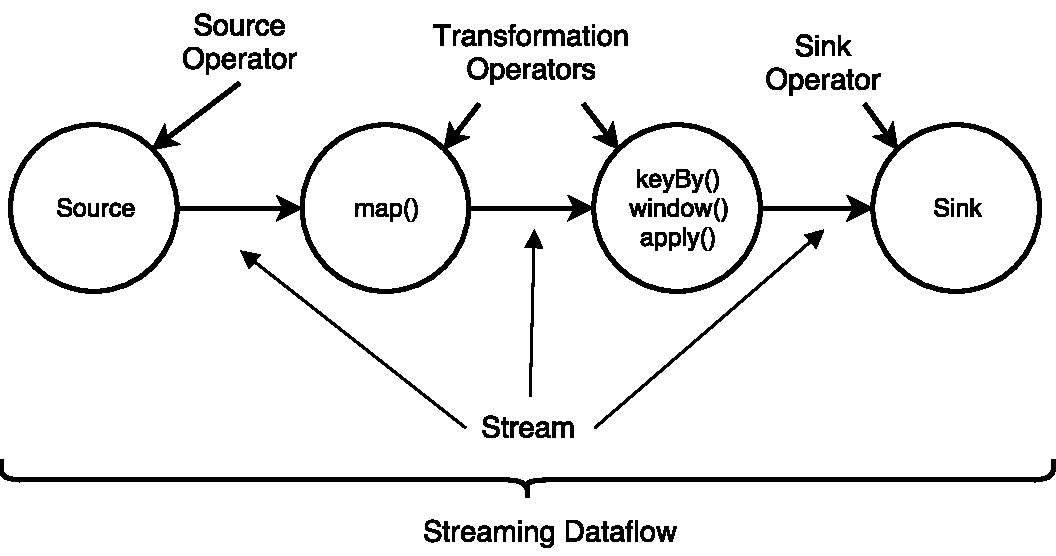
\includegraphics[scale=0.75]{Figures/dataflow.pdf}
	\decoRule
	\caption[Streaming Dataflow]{DAG outlining the previous code snippet}
	\label{fig:Dataflow}
\end{figure}

\paragraph{Event Time}

Flink supports different notions of time in streaming programs \cite{flink_eventtime} and each of them can be useful for specific use cases:

\begin{itemize}
    \item \textbf{Processing time} refers to the system time of the machine that is executing the respective operation.
    
    When it is being used, the system clock of the machines will be used to run all time-based operations. Being the simplest notion of time, no coordination between streams and machines is required, providing, this way, the best performance with the lowest latency. However, since the entire environment is distributed and can work asynchronously, processing time does not provide determinism, because of its susceptibility to the speed at which records arrive in the system and flow between each pair of operator inside the system.
    
    \item \textbf{Event time} is the time embedded within a record, representing when it occurred on its producing device. This time is typically assigned before records enter Flink and it can be extracted directly from the record. An event time window of an hour will contain only records carrying an event timestamp within that hour, regardless of their actual time and order of arrival.
    
    Event time is especially useful when dealing with out-of-order or late events, and even on replays of data from persistent logs or backups. When using event time, the progress of time is discretized based on the data, rather than the clock and, for this reason, the generation of the Event Time Watermarks, central to the mechanism that signals progress in event time,  must be specified internally to the program.
    
    Event time processing causes inherently a certain latency, due to its waiting for late and out-of-order events.
    
    \item \textbf{Ingestion time} is the time that events enter Flink. The source operator assigns to each record its current time as a timestamp, which all time-based operations refer to.
    
    Ingestion time can be considered an alternative sitting, conceptually speaking, in between event time and processing time: it is more expensive than processing time, while providing deterministic results, as it uses stable timestamps, assigned once at the source, used by all of the following time-based operations, but cannot handle any out-of-order events or late data, with respect to event time, even though there's no need to specify the watermarks generation.
\end{itemize}


\paragraph{Windows}

Windows are the core mechanism within a stream processing framework. They allow the application of operations after splitting the stream into \textit{buckets} of finite size. The structure of a windowed Flink program differs when considering \textbf{keyed} and \textbf{non-keyed} streams: a keyed stream is split into multiple logical sub-streams and a window is applied to each one of them separately, differently from a non-keyed stream where the window is applied globally and within a single task \cite{flink_windows}.

A Window lifecycle starts as soon as the first element belonging to it arrives and ends, being completely removed, when the time, event or processing time, passes its end timestamp plus any user-specified \textbf{allowed lateness}. For example, in an event-time-based Flink application where a tumbling window is created every 5 minutes with an allowed lateness of 1 minute, a new window will be created for the interval between 11:30 and 11:35, as soon as a record with a timestamp falling into that interval arrives, and will be removed when the watermark passes the 11:36 timestamp.

For each window must be specified a \textbf{Trigger} and a function (\texttt{WindowFunction}, \texttt{ReduceFunction} or \texttt{FoldFunction}) attached to it: the Trigger is used to specify the conditions under which the window is considered ready or complete for the function to be applied, while the function will contain the operation to be applied to the contents of the window. The triggering policy is completely customizable and can even decide to purge a window’s contents, leaving the window metadata untouched, in order to add new data to that window.

It's possible specify an \textbf{Evictor}, used to remove elements from the window after the trigger fires and before and/or after the function is applied.

There are four main window assigners usable in Flink:

\begin{itemize}
    \item \textbf{Tumbling Windows} are fixed size and non-overlapping windows, which are configured with a parameter controlling how much frequently a new window has to be started.
    \item \textbf{Sliding Windows} are fixed size, similarly to tumbling windows, but are configured with an additional slide parameter, which controls how frequently a sliding window is started. Therefore they overlap and elements are assigned to multiple windows.
    \item \textbf{Session Windows} group elements by sessions of activity. Session windows do not overlap and do not have a fixed start and end time, in contrast to tumbling windows and sliding windows. A session window closes when it does not receive elements for a certain period of time, i.e., when a gap of inactivity occurred.
    \item \textbf{Global Windows} assign all elements with the same key to the same single global window. This windowing scheme is only useful if you also specify a custom trigger. 
\end{itemize}



\paragraph{Parallelism} \label{ParallelismFlink}

Applications using Flink are inherently parallels and distributed. During execution, a stream may be divided in more than one partition; each operator can have more than a single sub-task operating on data, each one independent from the other and executed on different threads or, if possible, on different machines or containers.\\
The parallelism of a task is the parameter indicating the number of subtasks an operator can have and, consequentially, the number of partitions of the stream getting outputted from that operator.\\

\begin{figure}[!htb]
    \centering
    
\includegraphics[scale=0.75, trim=0.5cm 12cm 1cm 0.5cm]{Figures/parallel_dataflow.pdf}
    \decoRule
    \caption[Parallel Dataflow]{DAG with Parallelism=2}
    \label{fig:ParallelDataflow}
\end{figure}

Streams can transport data between a pair of operators following two different patterns: One-to-one pattern and redistributing pattern:
\begin{itemize}
	\item \textbf{One-to-one streams} preserve the stream partitioning and the order of the elements passed to the following operator. For example, the subtask[0] of a map() operator will get to see the same elements produced by the subtask[0] of the previous Source operator.
   
    \item \textbf{Redistributing streams} change their partitioning, sending the data to different subtasks, based on the transformation being applied. For example, a keyBy() operator repartitions the stream using the hash of the chosen key. In this case, the elements' order will be preserved only between neighbouring operations pairs, and won't be ever guaranteed being the same in the following operators.
\end{itemize}

\subsection{Data Streaming Fault Tolerance}

Flink offers built-in guarantees in case of failures, so that there's minimum disruption on the processing jobs and a consistent recovery of the data streaming applications' state. The two main features which allows recovery from errors or runtime exceptions are \textbf{Checkpoints} and \textbf{Savepoints}.

In case of a program failure (due to machine-, network-, or software failure), Flink stops the distributed streaming dataflow, restarting the operators and resetting them to the latest successful checkpoint, while also resetting the input streams to that same point of the state snapshot. Any records processed as part of the restarted parallel dataflow are guaranteed to not have been part of the previously checkpointed state.

For this mechanism to realize its full guarantees, the data stream source, being it a message queue or a broker, needs to be able to rewind the stream to a defined recent point. Apache Kafka, thanks to its offsets, has this ability and Flink’s connector to Kafka makes use of that ability.

\subsubsection{Checkpoints}

\begin{code}
    \label{code:checkpointing}
    \begin{minted}[breaklines, breakbefore=., breakafter=(]{Scala}
    val env: StreamExecutionEnvironment = StreamExecutionEnvironment.getExecutionEnvironment
    
    env.enableCheckpointing(60000)
    
    env.getCheckpointConfig.enableExternalizedCheckpoints(ExternalizedCheckpointCleanup.RETAIN_ON_CANCELLATION)
    
    env.setStateBackend(new FsStateBackend(state_dir, true)) 
    \end{minted}
    \captionof{listing}{An example of asynchronous checkpointing configuration on a FileSystem backend}
\end{code}~\\

\textbf{Checkpoints} are Flink's tool to guarantee automatic fault tolerance and recovery of the job's state, in case of runtime errors or failures \cite{flink_checkpointing}. 
\\
\\
They are, essentially, snapshots of the current state of the job that act consistently as the system fall back in case of failure. Flink’s mechanism for drawing these snapshots is inspired by the standard Chandy-Lamport algorithm \cite{Chandy:1985:DSD:214451.214456} for distributed snapshots and is specifically tailored to Flink’s execution model \cite{DBLP:journals/corr/CarboneFEHT15}. 
\\
\\
Checkpointing must be configured on the application level as shown in the previous snippet by calling the \texttt{enableCheckpointing(milliseconds)} to specify how much time should pass between two consecutive snapshots. By default, if a job is cancelled the checkpoint is deleted as well, so the retainment on cancellation must be enabled manually. 
\\
\\
An additional configuration available to application level setup is the State Back-end, that is the location where the checkpoint, thus, the job's state, should be saved. There are three possible back-ends which can be chosen from: \textbf{in Memory}, useful for testing, on a \textbf{Filesystem} (local or distributed, like HDFS) and on \textbf{RocksDB}\footnote{\href{http://rocksdb.org/}{RocksDB} is an embeddable persistent key-value store for fast storage}, particularly recommended for huge states. Optionally, snapshots can be taken asynchronously in order not to block the processing pipeline.
Checkpoints can be used to manually recover from failures through specific commands from Flink CLI, but they don't support scaling on recovery, that is, parallelism can't be changed when recovering from a snapshot.

\paragraph{Barriers}

A core element in Flink’s distributed checkpointing are the \textit{stream barriers}: lightweight elements flowing with the records, as part of the data stream, injected into the stream starting from the data source, without interrupting it. They are used to separate the records in the data stream belonging to two consecutive snapshots. Each barrier contains the ID of the snapshot whose records were pushed in front of it: there can be multiple barriers belonging to different snapshots, meaning that checkpoints may happen concurrently.
\\
\begin{figure}[!htb]
    \centering
    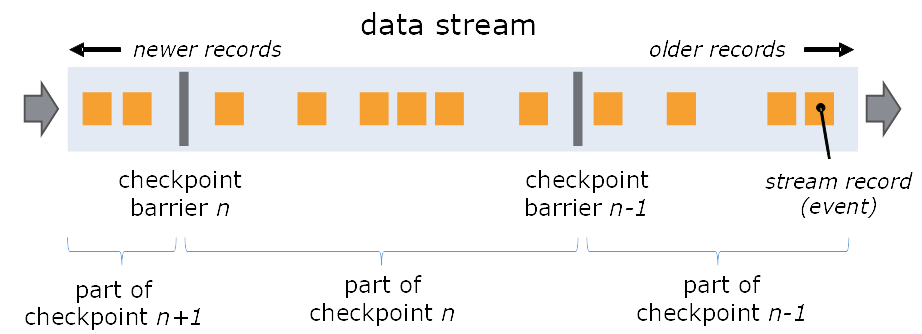
\includegraphics[width=1\linewidth]{Figures/stream_barriers}
    \caption{Visual representation of Stream Barriers}
    \label{fig:streambarriers}
\end{figure}
\\
Let's call $S_n$ the point in the stream where the barriers for snapshot $n$ are injected, representing the position up to which the snapshot covers the data, reported to the checkpoint coordinator, Flink’s JobManager.
\\\\
Flowing downstream, each intermediate operator must receive a barrier for snapshot $n$ from all of its input streams before, then, emitting a barrier for the same snapshot into all of its outgoing streams, until a sink operator is reached. Once a sink has received a barrier $n$, from all of its input streams, the snapshot $n$ is acknowledged to the checkpoint coordinator and the checkpoint is considered complete.

At the completion of snapshot $n$, the job will never ask the sources to replay the records from before $S_n$, since they all went through the topology.
\\\\

If an operator receives more than one input stream, an \textit{\textbf{alignment}} step must be performed between all of the inputs:

\begin{itemize}
\item As soon as the operator has received a snapshot barrier $n$ from an incoming stream, it must wait the same barrier from all of the other inputs, since otherwise processing would mix records belonging to consecutive snapshots and, in this case, would use also the barriers for snapshot $n+1$.

\item While waiting, all barriers $n$ are temporarily set aside and the corresponding records put in an input buffer.
    
\item Once the last stream has received barrier $n$, the operator emits all pending outgoing records and then snapshot $n$ barriers itself, before continuing processing records, starting from input buffers and then the actual input streams.
\end{itemize}

\paragraph{Exactly Once vs. At Least Once}

The alignment step previously described may add latency to the streaming program, usually negligible, being in the the order of a few milliseconds, but some applications' latency may increase noticeably. If consistent super low latency (few milliseconds) for all records is a strict requirement, Flink allows to skip the stream alignment during a checkpoint, but snapshots are still drawn as soon as an operator has seen the checkpoint barrier from each input stream.

As a consequence, the operator keeps processing all inputs, including elements belonging to checkpoint $n+1$, which will then occur as duplicates when restoring the state of the stream because they are both included in the state snapshot of checkpoint $n$ and part of the data following this same checkpoint.
\\

The alignment step happens only when operators with multiple predecessors (join operators) or 
multiple senders (such as a stream repartitioning/shuffle) are present. For this reason, dataflows containing only parallel streaming operations (\texttt{map()}, \texttt{flatMap()}, \texttt{filter()}, …) guarantee \textit{exactly once} semantics even in \textit{at least once} mode.

\subsubsection{Savepoints}

\begin{code}
    \label{code:savepoint}
    \begin{minted}{Bash}
flink savepoint <jobId> [<savepointDirectory>] -yid <yarnAppId> 
    \end{minted}
    \captionof{listing}{Savepoint triggering from the Flink CLI}
\end{code}~\\

\textbf{Savepoints}, just like checkpoints, serve the purpose to save the state of a Flink application in case of cancellation or failures. Differently from checkpoints, they can only be performed manually from Flink CLI, but support parallelism rescaling and they're the go-to choice when Flink's application computational capabilities must be improved by setting an higher parallelism factor or when an upgrade to a more recent version of Flink must be performed. Savepoint's mechanism works such that it associates each application's stateful operator, to its own state in a map-like structure: for this very reason, in order to successfully preserve state when upgrading a Flink application, each stateful operator needs to have its own \texttt{uid} set.

\subsection{High Availability}

A Flink's setup, whether a standalone cluster (being it containerized or physical) or using Distributed Resource Managers such as \nameref{YARN} or Mesos\footnote{\href{https://mesos.apache.org/}{Mesos} is a distributed cluster manager used to manage datacenters with a master-slave architecture. It's a lower level abstraction with respect to YARN and thus performs a different job more inclined towards machines management and task scheduling, than purely job's scheduling.}, is made of a Job Manager and one or more Task Managers, each one with one or more parallelism slots (cores usable for processing). Task Managers (TMs) handle jobs actual executions, while the Job Manager (JM) handles TM orchestration and monitoring and, for this reason, is a single point of failure, whose crash causes the entire Flink cluster to stop.
follows the principles of a Active-Standby architecture (also used by HDFS Namenode e YARN Resource Manager HA set-ups) where a single leading JM is active, while multiple JMs standby, ready to take over leadership in case the leader failure. This guarantees that there is no single point of failure and programs can make progress as soon as a standby JM has taken leadership. There is no explicit distinction between standby and master JM instances: all of the possible JMs are registered as masters to \textbf{Zookeeper}, which is going to handle failure scenarios.

In case of YARN clusters configured in High Availability mode, a single JM, being the \textbf{Application Master}, is still run, but YARN itself will restart its container on failures. As additional configuration, the maximum number of attempts for the application masters needs to be configured in the YARN configuration.

\subsection{Flink Extensions} \label{FlinkLibs}

\subsubsection{FlinkCEP: Complex Events Processing}

FlinkCEP is a Flink extension adding the possibility to analyse events pattern in a DataStream, thanks to the Pattern API. This API allows the definition of patterns to be found in a stream and their selection in order to create a new DataStream of Alerts.\\


\begin{code}
\label{code:pattern-example}
\begin{minted}[breaklines]{Scala}

val inputStream: DataStream[SensorEvent] = ...

val pattern = Pattern.begin("start").where(_.getId == 42)
.next("middle").subtype(classOf[TemperatureEvent]).where(_.getTemperature >= 90.0)
.followedBy("end").where(_.getName == "end")

val patternStream = CEP.pattern(inputStream, pattern)

val result: DataStream[Alert] = patternStream.select(createAlert(_))
\end{minted}
\captionof{listing}{An example of Pattern API usage}
\end{code}~\\

In FlinkCEP, a \textbf{Pattern}, similarly to a pattern of a Regular Expression, can be \textbf{single} or \textbf{iterative}. For example, in a pattern like \texttt{"a b+ c? d"}, \texttt{a}, \texttt{c?} e \texttt{d} are single patterns, while \texttt{b+} is iterative.
\\

In a Pattern there can be, analogously to Regular Expressions, Quantifiers and Conditions.

\paragraph{Quantifiers}

Iterative patterns can be specified with the following self explanatory methods:

\begin{itemize}
    \item \texttt{pattern.oneOrMore()};
    \item \texttt{pattern.times(\#ofTimes)};
    \item \texttt{pattern.optional()}
\end{itemize}

\paragraph{Conditions}

Each pattern can have additional conditions specified, which can be related to a property of an incoming event, or the contiguity to other events.

Methods \texttt{pattern.where()} and \texttt{pattern.or()} can be used to specify \texttt{\justify{IterativeCondition}}s, \texttt{SimpleCondition}s or a combination of multiple conditions. In this case, combinations can be specified concatenating all the previous methods, including the quantifiers, optionally adding more constraints on the contiguity of the same pattern by calling \texttt{consecutive()}, for the strict contiguity, and \texttt{allowCombinations()} for the relaxed non-deterministic contiguity.
\\
Some examples:

\begin{code}
\label{code:iterative-cond}
\begin{minted}[breaklines]{Scala}
middle.oneOrMore().where(
    (value, ctx) => {
        lazy val sum = ctx.getEventsForPattern("middle")
                          .asScala.map(_.getPrice).sum
        value.getName.startsWith("foo") && sum + value.getPrice < 5.0
    }
)
\end{minted}
\captionof{listing}{Iterative Condition}
\end{code}~\\

\begin{code}
    \label{code:simple-cond}
    \begin{minted}[breaklines]{Scala}
//Example of conjunction through where concatenation
start.where(event => event getName startsWith "foo" ) )
     .where(event => event getTotal equals 50  )

start.subtype(classOf[SubEvent]).where(subEvent => ... /* some condition */)
    \end{minted}
    \captionof{listing}{Conditions combinations}
\end{code}~\\

\paragraph{Pattern Combination}

Similarly to conditions combination, pattern combination is possible through the consecutive calls to the following methods allowing to specify the contiguity constraints which a given pattern should satisfy:

\begin{itemize}
    
    \item \texttt{next()}, for strict contiguity.
    \item \texttt{followedBy()}, for relaxed contiguity.
    \item \texttt{followedByAny()}, for non deterministic relaxed contiguity.
    \item \texttt{notNext()}, NOT pattern with strict contiguity.
    \item \texttt{notFollowedBy()}, NOT pattern with relaxed contiguity.

\end{itemize}

Each pattern combination can be followed by a time constraint specified by concatenating \texttt{within(Time)}.

\paragraph{Pattern Detection}

Once a pattern sequence has been specified, it needs to applied to the target \texttt{Datastream}, creating this way a \texttt{PatternStream}.
On this new stream \texttt{select} or \texttt{flatSelect} operations need to be applied in order to enable further processing on the events satisfying the pattern.

\subsubsection{Other extensions: Flink Gelly and FlinkML}

In addition to the aforementioned library for complex event handling, Flink makes specific sets of API available, which provide useful tools when it comes to enable advanced processing on data.

\paragraph{Flink Gelly} is an API based on the Flink \texttt{Dataset}s API specifically developed for Graph Processing. Graphs are stored as a finite set of vertices and edges, a special case of a \texttt{Dataset}. This library allows the application of operators like Map, Filter, Intersect and Union, Mutations like edge and vertex removal, but also advanced techniques belonging to Graph Theory like \textit{Iterative Graph Processing} (Vertex-centric, Scatter-Gather and Gather-Sum-Apply), \textit{Single Source Shortest Paths}, \textit{Clustering} and Similarity analysis.

\paragraph{FlinkML} is a set of tools which allows the application of Machine Learning techniques on Flink data streams, including both algorithmic implementations for supervised (\textit{SVMs} and \textit{Multiple Linear Regressors}) and unsupervised (\textit{K-nearest neighbours}) learning, Data Preprocessing and Recommendation (\textit{ALS}).



%\include{Chapters/Chapter4} 
%\include{Chapters/Chapter5} 

%----------------------------------------------------------------------------------------
%	THESIS CONTENT - APPENDICES
%----------------------------------------------------------------------------------------

\appendix % Cue to tell LaTeX that the following "chapters" are Appendices

% Include the appendices of the thesis as separate files from the Appendices folder
% Uncomment the lines as you write the Appendices

% Appendix A

\chapter{Frequently Asked Questions} % Main appendix title

\label{AppendixA} % For referencing this appendix elsewhere, use \ref{AppendixA}

\section{How do I change the colors of links?}

The color of links can be changed to your liking using:

{\small\verb!\hypersetup{urlcolor=red}!}, or

{\small\verb!\hypersetup{citecolor=green}!}, or

{\small\verb!\hypersetup{allcolor=blue}!}.

\noindent If you want to completely hide the links, you can use:

{\small\verb!\hypersetup{allcolors=.}!}, or even better: 

{\small\verb!\hypersetup{hidelinks}!}.

\noindent If you want to have obvious links in the PDF but not the printed text, use:

{\small\verb!\hypersetup{colorlinks=false}!}.

%\include{Appendices/AppendixB}
%\include{Appendices/AppendixC}

%----------------------------------------------------------------------------------------
%	BIBLIOGRAPHY
%----------------------------------------------------------------------------------------

\printbibliography[heading=bibintoc]

%----------------------------------------------------------------------------------------

\end{document}  
